\documentclass[xcolor=pdflatex,dvipsnames,table]{beamer}
\usepackage{epsfig,graphicx}
\usepackage{palatino}
\usepackage{fancybox}
\usepackage{relsize}
\usepackage[procnames]{listings}
\usepackage{hyperref}
\usepackage{qtree} % needed?
\usepackage{booktabs}
\usepackage{dirtree}
\usepackage[normalem]{ulem}


% fatter TT font
\renewcommand*\ttdefault{txtt}
% another TT, suggested by Alex
% \usepackage{inconsolata}
% \usepackage[T1]{fontenc} % needed as well?


\newcommand{\scale}{0.7}

\newcommand{\todo}[1]{{\emph{TODO: #1}}}
\newcommand{\martin}[1]{{\color{blue} Martin: #1}}
\newcommand{\abcdef}[1]{{\color{red} Author2: #1}}

% uncomment following for final submission
%\renewcommand{\todo}[1]{}
%\renewcommand{\martin}[1]{}
%\renewcommand{\author2}[1]{}

\newcommand{\code}[1]{{\texttt{#1}}}

\hypersetup{
  linkcolor  = black,
%  citecolor  = blue,
  urlcolor   = blue,
  colorlinks = true,
}

\beamertemplatenavigationsymbolsempty
\setbeamertemplate{footline}[frame number]





\newif\ifbook
% shared in slides and book

\lstdefinelanguage{chisel}{
  morekeywords={abstract,case,catch,class,def,%
    do,else,extends,false,final,finally,%
    for,if,implicit,import,match,mixin,%
    new,null,object,override,package,%
    private,protected,requires,return,sealed,%
    super,this,throw,trait,true,try,%
    type,val,var,while,with,yield},
  otherkeywords={=>,<-,<\%,<:,>:,\#,@},
  sensitive=true,
  morecomment=[l]{//},
  morecomment=[n]{/*}{*/},
  morestring=[b]",
  morestring=[b]',
  morestring=[b]"""
}

\usepackage{color}
\definecolor{dkgreen}{rgb}{0,0.6,0}
\definecolor{gray}{rgb}{0.5,0.5,0.5}
\definecolor{mauve}{rgb}{0.58,0,0.82}

% Default settings for code listings
\ifbook
\lstset{%frame=lines,
  language=chisel,
  aboveskip=3mm,
  belowskip=3mm,
  showstringspaces=false,
  columns=fixed, % basewidth=\mybasewidth,
  basicstyle={\small\ttfamily},
  numbers=none,
  numberstyle=\footnotesize,
  % identifierstyle=\color{red},
  breaklines=true,
  breakatwhitespace=true,
  procnamekeys={def, val, var, class, trait, object, extends},
  % procnamestyle=\ttfamily,
  tabsize=2,
  float
}
\else
\lstset{%frame=lines,
  language=chisel,
  aboveskip=3mm,
  belowskip=3mm,
  showstringspaces=false,
  columns=fixed, % basewidth=\mybasewidth,
  basicstyle={\small\ttfamily},
  numbers=none,
  numberstyle=\footnotesize\color{gray},
  % identifierstyle=\color{red},
  keywordstyle=\color{blue},
  commentstyle=\color{dkgreen},
  stringstyle=\color{mauve},
  breaklines=true,
  breakatwhitespace=true,
  procnamekeys={def, val, var, class, trait, object, extends},
  procnamestyle=\ttfamily\color{red},
  tabsize=2,
  float
}
\fi

\lstnewenvironment{chisel}[1][]
{\lstset{language=chisel,#1}}
{}

\newcommand{\shortlist}[1]{{\lstinputlisting[nolol]{#1}}}

\newcommand{\longlist}[3]{{\lstinputlisting[float, caption={#2}, label={#3}, frame=tb, captionpos=b]{#1}}}

\newcommand{\verylonglist}[3]{{\lstinputlisting[caption={#2}, label={#3}, frame=tb, captionpos=b]{#1}}}


\title{Chisel Basic Operations}
\author{Martin Schoeberl}
\date{\today}
\institute{Technical University of Denmark}

\begin{document}

\begin{frame}
\titlepage
\end{frame}

\begin{frame}[fragile]{Chisel Data Types}
\begin{itemize}
\item Data types for values on wires or state elements
\item Raw collection of bits is type \code{Bits}
\item Simple types to represent integer numbers
\begin{itemize}
\item Unsigned and signed
\item Subtype of \code{Bits}
\end{itemize}
\item \emph{Interesting} way to specify constants
\item Automatic bit width inference
\item Boolean values are of type \code{Bool}, a single bit value
\end{itemize}
\begin{chisel}
1.U
"habcd".U
"b0101".U
-5.S
true.B
\end{chisel}
\end{frame}

\begin{frame}[fragile]{Chisel Data Types}
\begin{itemize}
\item Bit width can be explicitly specified with a width type
\begin{itemize}
\item \code{SInt} will be sign extended
\item \code{UInt} will be zero extended
\end{itemize}
\end{itemize}
\begin{chisel}
0.U(32.W)
"habcd".U(24.W)
-5.S(16.W)
\end{chisel}
\begin{itemize}
\item \emph{Bundles} for a named collection of values
\item \emph{Vecs} for indexable collection of values
\item Chisel data types are different from Scala builtin types (e.g., Scala's \code{Int})
\end{itemize}
\end{frame}

\begin{frame}[fragile]{Bitwise Logical Operations}
\begin{itemize}
\item Bitwise NOT, AND, OR, and XOR
\item Automatic size extension to larger operand
\end{itemize}
\begin{chisel}
val notVal = ~x
val maskOut = x & "b00001111".U
val orVal = x | y
val xorVal = x ^ y
\end{chisel}
\begin{itemize}
\item Bit reduction
\item Results in a single bit
\end{itemize}
\begin{chisel}
x.andR
x.orR
x.xorR
\end{chisel}
\end{frame}

\begin{frame}[fragile]{Arithmetic Operations}
\begin{itemize}
\item Addition, subtraction, multiplication, division, modulos
\item Automatic size extension to larger operand
\end{itemize}
\begin{chisel}
+, -, *, /, %
\end{chisel}
\begin{itemize}
\item Left and right shifts
\item Left shift extends bit width
\item Right shift reduces bit width
\end{itemize}
\begin{chisel}
<<, >>
\end{chisel}
\end{frame}

\begin{frame}[fragile]{Bitfield Manipulations}
\begin{itemize}
\item Extract a single bit
\end{itemize}
\begin{chisel}
val sign = x(31)
\end{chisel}
\begin{itemize}
\item Extract a sub field from end to start position
\end{itemize}
\begin{chisel}
val lowByte = word(7, 0)
\end{chisel}
\begin{itemize}
\item Concatenate bit fields
\end{itemize}
\begin{chisel}
val word = Cat(highByte, lowByte)
\end{chisel}
\end{frame}

\begin{frame}[fragile]{Comparison}
\begin{itemize}
\item The usual operations
\begin{itemize}
\item Unusual equal and unequal operator symbols
\item To keep the original Sala operators usable for references
\end{itemize}
\item Operands are \code{UInt} and \code{SInt}
\item Operands can be \code{Bool} for equal and unequal
\item Result is \code{Bool}
\end{itemize}
\begin{chisel}
===, =/=
>, >=, <, <=
\end{chisel}
\end{frame}

\begin{frame}[fragile]{Boolean Logical Operations}
\begin{itemize}
\item Operands and result are \code{Bool}
\item Logical NOT, AND, and OR
\end{itemize}
\begin{chisel}
val notX = !x
val bothTrue = a && b
val orVal = x || y
\end{chisel}
\end{frame}

\begin{frame}[fragile]{Combinational Circuits}
\begin{itemize}
\item Circuit is a graph of nodes
\item A node is a hardware operator with zero or more inputs
\item Textual expression to wire up nodes
\item Named wires with some (unspecified) width
\end{itemize}
\begin{chisel}
(a | b) & ~c
\end{chisel}
\end{frame}

\begin{frame}[fragile]{Combinational Circuits}
\begin{itemize}
\item Simple expressions represent a circuit tree
\item Arbitrary directed acyclic graphs need named subexpressions
\item Using Scala's \code{val} keyword for variables that don't change
\item Referenced multiple times
\end{itemize}
\begin{chisel}
val cond = a & b
val result = (cond & selA) | (!cond & selB)
\end{chisel}
\end{frame}

\begin{frame}[fragile]{Register}
\begin{itemize}
\item State elements
\item Has it's own Chisel type \code{Reg}
\item Positive edge triggered D flip-flop
\item Synchronous reset
\item Clock and reset are \emph{hidden wires}
\end{itemize}
\begin{chisel}
val q = RegNext(d)
\end{chisel}
\begin{itemize}
\item \code{d} is the input, \code{q} the output
\item Register type is inferred by the input (d) type
\end{itemize}
\end{frame}

\begin{frame}[fragile]{Register}
\begin{itemize}
\item Reset value as parameter on a \code{RegInit} constructor
\end{itemize}
\begin{chisel}
val initReg = RegInit(0.U(8.W))
\end{chisel}
\begin{itemize}
\item With this forward declaration we later assign the input
\end{itemize}
\begin{chisel}
initReg := initReg + 1.U
\end{chisel}
\begin{itemize}
\item A register can also be defined within an expression
\end{itemize}
\shortlist{../code/sequ_reg_rising.txt}
\end{frame}


\begin{frame}[fragile]{A Multiplexer}
\begin{figure}
  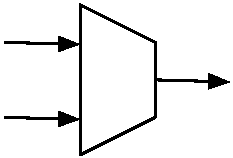
\includegraphics[scale=\scale]{../figures/mux}
\end{figure}
\begin{itemize}
\item A Multiplexer selects between alternatives
\item So common that Chisel provides a construct for it
\item Selects \code{a} when \code{sel} is \code{true.B} otherwise \code{b}
\item Could be implemented with conditional updates
\item Automagical type selection on input types
\end{itemize}
\shortlist{../code/mux.txt}
\end{frame}

\begin{frame}[fragile]{A Small Circuit}
\begin{itemize}
\item Our Chisel knowledge is complete enough\\ to implement any digital circuit
\item Maybe not in the most elegant way ;-)
\item A counter is a simple basic component
\item The following counts form 0 to 100
\end{itemize}
\begin{chisel}
  val cntReg = RegInit(0.U(8.W))

  cntReg := Mux(cntReg === 100.U,
    0.U, cntReg + 1.U)
\end{chisel}
\end{frame}

\begin{frame}[fragile]{The Complete Counter Module}
\begin{chisel}
class Counter extends Module {
  val io = IO(new Bundle {
    val cnt = Output(UInt(8.W))
  })

  val cntReg = RegInit(0.U(8.W))

  cntReg := Mux(cntReg === 100.U,
    0.U, cntReg + 1.U)

  io.cnt := cntReg
}
\end{chisel}
\end{frame}

\begin{frame}[fragile]{Data Aggregation}
\begin{itemize}
\item A \code{Bundle} groups several named fields
\item Like a C struct or VHDL record
\item \code{Vec} is a vector of elements with the same type
\item Can be arbitrary mixed
\end{itemize}
\begin{chisel}
class AluFields extends Bundle {
  val function = UInt(2.W)
  val inputA = UInt(8.W)
  val inputB = UInt(8.W)
  val result = UInt(8.W)
}
\end{chisel}
\end{frame}

\begin{frame}[fragile]{Vectors}
\begin{itemize}
\item Indexable vector of elements
\item Elements can be Chisel basic elements, or bundles
\item Type is specified as second parameter
\end{itemize}
\begin{chisel}
val myVec = Vec(3, SInt(10.W))
val y = myVec(2)
myVec(0) := -3.S
\end{chisel}
\begin{itemize}
\item A register file as a register of a vector
\end{itemize}
\begin{chisel}
val vecReg = Reg(Vec(32, SInt(32.W)))
\end{chisel}
\end{frame}

\begin{frame}[fragile]{Ports}
\begin{itemize}
\item Ports used to connect modules
\item Ports are bundles with directions
\end{itemize}
\begin{chisel}
class AluIO extends Bundle {
  val function = Input(UInt(2.W))
  val inputA = Input(UInt(4.W))
  val inputB = Input(UInt(4.W))
  val result = Output(UInt(4.W))
}
\end{chisel}
\end{frame}

\begin{frame}[fragile]{Port Directions}
\begin{itemize}
\item Can be assigned at instantiation
\end{itemize}
\begin{chisel}
class ExecuteIO extends Bundle {
  val dec = Input(new DecodeExecute())
  val mem = Output(new ExecuteMemory())
}
\end{chisel}
\begin{chisel}
\end{chisel}
\end{frame}

\begin{frame}[fragile]{Port Directions}
\begin{itemize}
\item Can be reversed with the \code{Flipped}
\item Convenient to have one bundle definition working as source
and destination used between two modules
\end{itemize}
\begin{chisel}
class Channel extends Bundle {
  val data = Input(UInt(32.W))
  val ready = Output(Bool())
  val valid = Input(Bool())
}

class ChannelUsage extends Bundle {
  val input = new Channel()
  val output = Flipped(new Channel())
}
\end{chisel}
\end{frame}

\begin{frame}[fragile]{Modules}
\begin{itemize}
\item Modules are used to organize the circuit
\item Similar to VHDL components (entity/architecture)
\item A class that inherits from \code{Module}
\item Circuit description in the constructor
\item Interface (port) is a \code{Bundle}, wrapped into an \code{IO()}, and stored in the field \code{io}
\end{itemize}
\begin{chisel}
class Adder extends Module {
  val io = IO(new Bundle {
    val a = Input(UInt(4.W))
    val b = Input(UInt(4.W))
    val result = Output(UInt(4.W))
  })

  val addVal = io.a + io.b
  io.result := addVal
}
\end{chisel}
\end{frame}

\begin{frame}[fragile]{Module Usage}
\begin{itemize}
\item Create with \code{new} and wrap into a \code{Module()}
\item Interface port via the \code{io} field
\item Note the assignment operator \code{:=} on \code{io} fields
\end{itemize}
\begin{chisel}
  val adder = Module(new Adder())
  adder.io.a := ina
  adder.io.b := inb
  val result = adder.io.result
\end{chisel}
\end{frame}

\begin{frame}[fragile]{Conditional Assignments}
\begin{itemize}
\item Conditional update of a value
\item Needs to be declared as a \code{Wire}
\item Last assignment counts
\item Is basically a multiplexer
\end{itemize}
\begin{chisel}
  val v = Wire(UInt())
  v := 5.U
  when (condition) {
    v := 0.U
  }

  when (c1) { v := 1.U }
  when (c2) { v := 2.U }
\end{chisel}
\end{frame}

\begin{frame}[fragile]{The Counter With a Conditional Update}
\begin{chisel}
class Counter2 extends Module {
  val io = IO(new Bundle {
    val cnt = Output(UInt(8.W))
  })

  val cntReg = RegInit(0.U(8.W))

  cntReg := cntReg + 1.U
  when (cntReg === 100.U) {
    cntReg := 0.U
  }

  io.cnt := cntReg
}
\end{chisel}
\end{frame}

\begin{frame}[fragile]{Chained Conditionals}
\begin{itemize}
\item Chain of conditionals with \code{.elsewhen}
\item With an optional \emph{else} path with \code{.otherwise}
\item Note that Scala has \code{if/else}
\begin{itemize}
\item Does NOT result in hardware
\item Are used to conditionally \emph{generate} hardware
\item We will look at this later
\end{itemize}
\item Note the ``.'' at the operators
\end{itemize}
\begin{chisel}
  when (c1) { v := 1.U }
  .elsewhen (c2) { v := 2.U }
  .otherwise { v := 3.U }
\end{chisel}
\end{frame}

\begin{frame}[fragile]{Switch Statement}
\begin{itemize}
\item Series of comparisons
\item Chisel allows combinational logic be updated conditionally 
\item Chisel disallows incomplete specified logic (= latches)
\item Chisel will report a runtime error
\end{itemize}
\begin{chisel}
  switch(fn) {
    is(0.U) { result := a + b }
    is(1.U) { result := a - b }
    is(2.U) { result := a | b }
    is(3.U) { result := a & b }
  }
\end{chisel}
\end{frame}

\begin{frame}[fragile]{More Chisel Example Code}
\begin{itemize}
\item The time-predictable processor Patmos
\item An SRAM controller for the DE2-115 board
\item An SSRAM controller
\item An UART
\item A memory arbiter
\item Caches
\item ...
\item \url{https://github.com/t-crest/patmos}
\end{itemize}
\end{frame}


\begin{frame}[fragile]{More Chisel Documentation}
\begin{itemize}
\item Textbook ``Digital Design with Chisel''
\item 2nd edition is out
\item \url{https://github.com/schoeberl/chisel-book}
\item Feedback is welcome
\item Contains all the slides
\end{itemize}
\end{frame}

\begin{frame}[fragile]{Chisel Tutorial from UCB}
\begin{itemize}
\item Collection of small exercises
\item Only in simulation, no hardware required (+/-)
\item All examples in \emph{one} design
\begin{itemize}
\item Results in a little bit more complex setup
\end{itemize}
\item Needs an Internet connection
\begin{itemize}
\item  Tests against latest Chisel version
\end{itemize}
\end{itemize}
\end{frame}

\begin{frame}[fragile]{Chisel Tutorial}
\begin{itemize}
\item Get the tutorial
\end{itemize}
\begin{chisel}
git clone https://github.com/ucb-bar/chisel-tutorial.git
cd chisel-tutorial
\end{chisel}
\begin{itemize}
\item Test the installation with a Hello World
\item Living in \code{src/main/scala/hello/Hello.scala}
\end{itemize}
\begin{chisel}
sbt run
\end{chisel}
\begin{itemize}
\item May take some time
\end{itemize}
\end{frame}

\begin{frame}[fragile]{Very Minimal Hello World}
\begin{chisel}
class Hello extends Module {
  val io = IO(new Bundle {
    val out = Output(UInt(8.W))
  })
  io.out := 42.U
}
\end{chisel}
\begin{itemize}
\item Produces hardware for a single constant
\end{itemize}
\end{frame}

\begin{frame}[fragile]{Testing the Minimal Hello World}
\begin{chisel}
class HelloTests(c: Hello) extends PeekPokeTester(c) {
  step(1)
  expect(c.io.out, 42)
}
\end{chisel}
\begin{itemize}
\item Drive the simulation with \code{step(1)}, which is a single clock tick
\item Test output against expected value
\end{itemize}
\end{frame}

\begin{frame}[fragile]{Tutorial Problems}
\begin{chisel}
sbt "test:runMain problems.Launcher Mux2"
\end{chisel}
\begin{itemize}
\item This example should already work
\item Read the hardware description and test code
\item Source organized in \code{main} and \code{test} folders
\item Problems and testers are in package/folder \code{problems}
\end{itemize}
\end{frame}

\begin{frame}[fragile]{Tutorial Problems}
\begin{chisel}
sbt "test:runMain problems.Launcher Mux4"
\end{chisel}
\begin{itemize}
\item The test should fail
\item Fix the Mux4 component so that the tests complete
\end{itemize}
\end{frame}

\begin{frame}[fragile]{Links to the Examples}
\begin{itemize}
\item Example code
\item \url{https://github.com/schoeberl/chisel-examples.git}
\end{itemize}
\end{frame}

\begin{frame}[fragile]{Lab Session}
\begin{itemize}
\item Run and explore the UART (serial port) example
\begin{itemize}
\item There is a make target that builds the UART hardware
\item \code{make uart}
\item It shall write some text out
\item You can observe it with a terminal (e.g., gtkterm)
\end{itemize}
\item Combine the UART with a blinking LED
\begin{itemize}
\item Write a `0' and `1' out on blink off and on
\item Best add the LEDs to \code{UartMain} and \code{uart\_top.vhdl}
\end{itemize}
\item Write repeated numbers 0--9 at maximum speed 
\end{itemize}
\end{frame}

%\begin{frame}[fragile]{More Problems}
%\begin{itemize}
%\item Explore more problems to solve
%\item Suggestions:
%\begin{itemize}
%\item Accumulator
%\item VecSchiftRegister (maybe)
%\end{itemize}
%\item Change the Blinking LED example so that
%\begin{itemize}
%\item It flashes for 1/5 second every second
%\end{itemize}
%\end{itemize}
%\end{frame}



\end{document}